\chapter{Modelo de Jaynes-Cummings}
\label{ch3_jcm}

%CAMBIAR ESTO PARA PERSONALIZARLO A MI GUSTO
\pagestyle{fancy}
\fancyhf{}
\fancyhead[LE]{\nouppercase{\rightmark\hfill}}
\fancyhead[RO]{\nouppercase{\leftmark\hfill}}
\fancyfoot[LE,RO]{\hfill\thepage\hfill}

En este capitulo analizaremos en profundidad la din\'amica y los aspectos teoricos mas importantes 
del modelo de Jaynes-Cummings, abordando el problema tanto desde un lado te\'orico, como desde
el lado computacional, necesario para resolver la din\'amica en sistemas abiertos.
Primero se trabajar\'a en el modelo de un átomo en una cavidad, se analizar\'an los casos importantes,
y se explicar\' la din\'amica del problema. Esto es importante para comprender conceptualmente como
interact\'uan fundamentalmente la materia y la luz, y nos sirve para conseguir buena intuici\'on del
problema de dos átomos. Tambien se ver\'a la influencia del entorno sobre la cavidad, permitiendo
perdida (o absorci\'on) de fotones, y tambien el bombeo coherente que puede excitar espontaneamente
al átomo. \newline

\section{Modelo y aproximaciónes}
Comencemos entonces por el paradigmatico modelo de 1 átomo. El modelo de Jaynes-Cummings consiste en describir la interacción entre la materia y la luz de manera cuantica, y el experimento mas sencillo consta de un átomo de dos niveles atrapada en una cavidad. La simpleza del modelo surge de las aproximaciónes e hipotesis que se hacen, en primer lugar, el campo electromagnetico dentro de la cavidad puede en principio tener infinitos modos, pero para simplificar se considera solo un modo. 
Entonces tenemos un Hamiltoniano ($\hbar = 1$)

\begin{align*}
\hat H & = \hat H_A + \hat H_C + \hat H_{int}  \\
\hat H_A &= \omega \frac{\sigma_z}{2} \\
\hat H_C &= \epsilon \hat a^\dagger\hat a = \epsilon \hat n \\
\hat H_{int} &= -i g (\hat\sigma_-+\hat \sigma_+)(\hat a - \hat a^\dagger)
\end{align*}

donde $\epsilon$ y $\omega$ son las freccuencias naturales de la cavidad y del átomo respctivamente. Los operadores $\hat a$ y $\hat a^\dagger$ son los operadores de aniquilaci\'on y creaci\'on fot\'onicos de la cavidad y $\hat n =a^\dagger a$ es el operador de n\'umero de la cavidad, y $\hat \sigma_z$ es el operador de pauli. Los estados del átomo de dos niveles los llamamos $\ket{g}$ y $\ket{e}$ al estado ground y excitado respectivamente, y con esta notación los operadores $\sigma_\pm = (\sigma_x\pm i\sigma_y)/2$ son los operadores de subida y bajada atomicos. 
La interacci\'on es complicada, y para simplificar lo que se hace es usar la representaci\'on de interacci\'on, y uno encuentra que hay dos frecuencias, una que llamamos \textit{rotante} y es la diferencia entre las frecuencias caracteristicas $\epsilon-\omega$, y la otra frecuencia es la suma $\epsilon+\omega$. La aproximación de onda rotante vale cuando las frecuencias son similares $\epsilon\sim\omega$, y consta de despreciar la dinamica de los terminos contrarrotantes, ya que oscilan muy rapidamente en comparación con los terminos rotantes, y entonces podemos promediar los efectos de los terminos rapidos. Entonces al aplicar esta aproximación, justificada cuando $\epsilon\sim\omega$ y $g \ll \epsilon,\omega$ se obtiene el hamiltoniano de JC \ref{}\textcolor{red}{ludmi 49}
\begin{equation}
    H_{JC}=\epsilon a^\dagger a + \omega \sigma_z/2 + g(a^\dagger\sigma_-+a\sigma_+)
\end{equation} 
La interpretaci\'on de la interacci\'on en este caso es clara, las dos opciones son que el átomo suba un nivel de energ\'ia y en consecuencia la cavidad pierda un fot\'on, o que el átomo baje un nivel, y la cavidad gane una excitaci\'on. Este Hamiltoniano conserva el n\'umero total de excitaciones $\hat N= \hat n + \hat \sigma$. En este momento es usual aplicar una transformación unitaria $K=\exp{-i\omega t(a ^\dagger a + \sigma_z/2)}$ sobre el Hamiltoniano que queda 
\begin{equation}\label{eq3:hamiltoniano jcm}
    H=\frac{\Delta}{2}\sigma_z+g(a^\dagger \sigma_-+a \sigma_+)
\end{equation}
donde $\Delta = \epsilon - \omega$ es el \textit{detunning} entre las frecuencias de la cavidad y el átomo. Un ejemplo de esto es un átomo de Rydberg metido en una cavidad \ref{}, o ... \textcolor{red}{BUSCAR EJEMPLOS}.
Como el Hamiltoniano conserva la cantidad de excitaciones es oportuno agrupar los estados en funci\'on de la cantidad de excitaciones: $\{\ket{g,n},\ket{e,n-1}\}$. En esta base el Hamiltoniano se diagonaliza por bloques, ya que las interacciones conservan la cantidad total de excitaciones, entonces los elementos de matriz entre estados con diferente cantidad de excitaciones se corresponde
\begin{align*}
    [H,\hat N]=0 \implies & \bra{N'}H \hat N \ket{N} = \bra{N'}\hat N H \ket{N} \\
    & N \bra{N'}H  \ket{N} = N' \bra{N'}H \ket{N} \\
    & \implies \bra{N'}H \ket{N} = \begin{cases}
        0 \text{ , si } N' \neq N \\
        \bra{N}H \ket{N} \text{ , si } N'=N
    \end{cases}
\end{align*}
donde $\ket{N}$ es un estado con $N$ excitaciones totales. Entonces para resolver el problema solo tenemos que mirar el subespacio de 2x2 de n excitaciones, cuyo Hamiltoniano es
\begin{equation}
    H_n=\begin{pmatrix}
        -\frac{\Delta}{2} & g \sqrt{n} \\
        g \sqrt{n} & \frac{\Delta}{2} 
    \end{pmatrix}
\end{equation}
Resolvemos el problema de autovalores y autovectores y obtenemos
\begin{equation}
    \begin{aligned}
        \ket{\psi^n_-} & = \cos \frac{\theta_n}{2}\ket{g,n}-\sin \frac{\theta_n}{2}\ket{e,n-1} \\
        \ket{\psi^n_+} & = \sin \frac{\theta_n}{2}\ket{g,n}+\cos \frac{\theta_n}{2}\ket{e,n-1}        
    \end{aligned}
\end{equation}
con $E_{\pm}^n=\pm \frac{\Omega}{2}$ las autoenergias y $\Omega_n=\sqrt{\Delta^2+4g^2n}$ la frecuencia de Rabi del sistema, $\cos \theta_n=\frac{\Delta}{\Omega_n}$ modulando la superposici\'on de estados. 
\begin{figure}
    \centering
    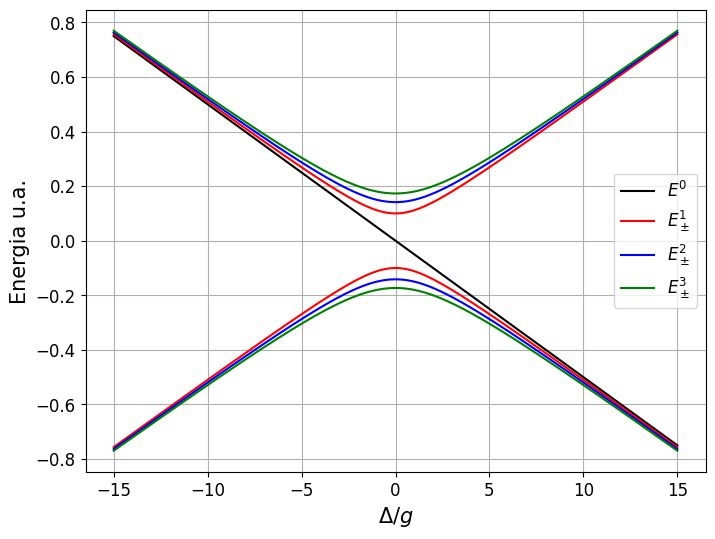
\includegraphics[width=0.7\textwidth]{figuras/ch3/relacion energia detunning jcm simple.png}
    \caption{Relaci\'on energ\'ia detunning para el modelo de Jaynes-Cummings. La diferencia de energ\'ia entre los estados de un mismo nivel para $\Delta=0$ es $2g\sqrt{n}$.}
    \label{fig:relación energia detunning jcm1}
\end{figure}
En la figura \ref{fig:relación energia detunning jcm1} se observan las curvas de energ\'ia en funci\'on del detunning para diferentes niveles. Lo primero que tenemos que observar es que en el caso resonante, es decir $\Delta=0$, los autoestados del sistema son los estados maximamente entrelazados de Bell
\begin{equation}
    \ket{\psi_\pm^n}=\frac{1}{\sqrt{2}}(\ket{gn}\pm\ket{e,n-1})
\end{equation} 
y la diferencia de energ\'ia entre los autoestados es $\Delta E^n =E^n_+-E^n_-=2g\sqrt{n}$. En el caso muy lejos de resonancia podemos asumir que $\Delta \gg g $, y entonces los autoestados coinciden en este l\'imite con los estados de la base, 
\begin{equation}
    \begin{aligned}
        \ket{\psi^n_+}=\ket{e,n-1} \\
        \ket{\psi^n_-}=\ket{g,n}
    \end{aligned}
\end{equation}
Ac\'a hay una sutileza, y es que si $\Delta>0$, entonces $\ket{e,n-1}$ es el estado de mayor energ\'ia y la notaci\'on coincide con la energ\'ia, pero si $\Delta<0$ entonces el estado $\ket{\psi^n_+}$ es el estado de menor energ\'ia. 
Un efecto interesante es que en el caso de alta desinton\'ia, podemos calcular la diferencia entre la energía del autoestado exacto del Hamiltoniano $\ket{\psi_\pm^n}$ y la energía asintotica a la que tiende, que es la energía de los estados de la base $\ket{g,n},\ket{e,n-1}$. Esta diferencia ... \textcolor{red}{VOLVER A ESTO Y VER SI DEJARLO O SACARLO. EVENTUALMENTE COMPLETAR.}
\begin{equation}
    \begin{aligned}
        \Delta E_{e,n-1}=E_+^n-E^{(0)}_{e,n-1}=\frac{g^2}{\Delta}n
        \Delta E_{g,n}=E_-^n-E^{(0)}_{g,n}=-\frac{g^2}{\Delta}n
    \end{aligned}
\end{equation}
El resultado importante de esta diferencia de energias es que aun en ausencia de fotones en la cavidad $n=0$, hay una diferencia entre las energias entre el Hamiltoniano del átomo, y del $H_{JC}$. Este efecto es el \textit{Lamb Shift} y nos dice que el vac\'io electromagnetico induce un corrimiento en la energ\'ia de los estados. Esto es importante notarlo, porque para el caso de dos átomos tambien est\'a manifiesto.

\subsection{Fase geométrica en el JCM}
Vamos a analizar la fase de Berry y la fase geométrica en la aproximación cinemática.
\subsubsection{Fase de Berry}
Para ver la fase de berry tenemos que tener un parámetro de control en el Hamiltoniano, el cual varía lentamente. Para esto necesitamos aplicar una transformación unitaria de corrimiento de fase al Hamiltoniano original \ref{eq3:hamiltoniano jcm} $R=\exp{-i\Omega a^\dagger a}$, que queda
\begin{equation}
    H=\frac{\Delta}{2}\sigma_z+g(a^\dagger \sigma_e^{-i\Omega}-+a\sigma_+e^{i\Omega})
\end{equation}
que ahora depende explicitamente del parámetro externo de control $\Omega$. Los autoestados de este nuevo Hamiltoniano se obtienen aplicando esta misma transformación sobre los autoestados del Hamiltoniano original. Si el parámetro de control varia lentamente entre 0 y $2\pi$, entonces estamos dentro de las hipotesis propuestas por Berry, y podemos calcular la fase de Berry mediante la ecuación \ref{eq2:fg berry}:
\begin{equation}
    \psi_a^n=i\oint_Cd\Omega\bra{\psi_\pm^n}R(\Omega)^\dagger \frac{d}{d\Omega}\ket{\psi_\pm^n}=\pi(1\pm \cos(\theta_n))
\end{equation}

que es no trivial incluso para $n=0$, lo que nos dice que incluso el vacio electromagnetico introduce una corrección en la fase de Berry.
\subsubsection{aproximación cinemática}
Para comparar ambos metodos, ahora vamos a calcular la fase geométrica utilizando la aproximación cinemática aunque este abordaje es más general de lo necesario en este caso.
Si se considera que el estado inicial es un atuoestado del Hamiltoniano, como los estados $\ket{\psi_\pm^n}$, entonces la fase geométrica en este caso se anula. Pero si se considera un estado inicial, por ejemplo $\ket{\psi(0)}=\ket{e,n}$, entonces el estado a tiempo $t$ resulta
\begin{equation}
    \ket{\psi(t)}=(\cos^2\theta_ne^{-iE_+^nt}+\sin^2\theta_ne^{iE_+^nt})\ket{e,n}-i \sin\theta_n\sin(E_+^nt)\ket{g,n+1}
\end{equation}
La fase geometrica acumulada \ref{eq2:fg cinematica unitaria} es
\begin{equation}
    \phi_u[C]=-\pi(1-\cos\theta_n)\frac{t}{T} +\arg\left\{ 1+e^{2\pi i \frac{t}{T}\frac{\Omega_n-\Delta}{\Omega_n+\Delta}} \right\}
\end{equation}
